% 
% Lecture Template for ME3050 -  Dynamics Modeling and Controls - Tennessee Technological University
%
% Spring 2020 - Summer 2020
% Tristan Hill, May 07, 2020
% Module 3 - Energy Methods
% Topic 1 - 
%

\documentclass{beamer}                         % for presentation (has nav buttons at bottom)
%\documentclass[handout]{beamer}  % for handout 
\usepackage{beamerthemesplit}
\usepackage{amsmath}
\usepackage{listings}
\usepackage{multicol}
\usepackage{framed}

\beamertemplateballitem

% custom colors
\definecolor{TTUpurple}{rgb}{0.3098, 0.1607, 0.5176} % TTU Purple (primary)
\definecolor{TTUgold}{rgb}{1.0000, 0.8666, 0.0000} % TTU Gold (primary) 
\definecolor{mygray}{rgb}{.6, .6, .6}
\definecolor{mypurple}{rgb}{0.6,0.1961,0.8}
\definecolor{mybrown}{rgb}{0.5451,0.2706,0.0745}
\definecolor{mygreen}{rgb}{0, .39, 0}
\definecolor{mypink}{rgb}{0.9960, 0, 0.9960}

% color commands
\newcommand{\R}{\color{red}}
\newcommand{\B}{\color{blue}}
\newcommand{\BR}{\color{mybrown}}
\newcommand{\K}{\color{black}}
\newcommand{\G}{\color{mygreen}}
\newcommand{\PR}{\color{mypurple}}
\newcommand{\PN}{\color{mypink}}
\newcommand{\OR}{\color{TTU}}
\newcommand{\GD}{\color{TTUgold}}


\setbeamercolor{palette primary}{bg=TTUpurple,fg=TTUgold}
\setbeamercolor{palette secondary}{bg=black,fg=TTUgold}
\setbeamercolor{palette tertiary}{bg=black,fg=TTUpurple}
\setbeamercolor{palette quaternary}{bg=TTUgold,fg=black}
\setbeamercolor{structure}{fg=TTUpurple} % itemize, enumerate, etc
\setbeamercolor{section in toc}{fg=TTUpurple} % TOC sections

%\usefonttheme{professionalfonts}

\newcommand{\LNUM}{3\hspace{2mm}} % Lecture Number 

\newcommand{\Lagr}{\mathcal{L}} % lagrangian

\newcommand{\hspcu}{\underline{\hspace{20mm}}} % large horizontal space w underline
\newcommand{\vspccc}{\vspace{6mm}\\} % large vertical space
\newcommand{\vspcc}{\vspace{4mm}\\}   % medium vertical space
\newcommand{\vspc}{\vspace{2mm}\\}     % small vertical space

\newcommand{\hspcccc}{\hspace{10mm}} % large horizontal space
\newcommand{\hspccc}{\hspace{6mm}} % large horizontal space
\newcommand{\hspcc}{\hspace{4mm}}   % medium horizontal space
\newcommand{\hspc}{\hspace{2mm}}     % small horizontal space

\author{ME3050 - Dynamics Modeling and Controls} % original formatting from Mike Renfro, September 21, 2004

\newcommand{\MNUM}{4\hspace{2mm}} % Module number
\newcommand{\TNUM}{3\hspace{2mm}} % Topic number 
\newcommand{\moduletitle}{Energy Methods }
\newcommand{\topictitle}{Example: Swinging Pendulum} 

\newcommand{\sectiontitleI}{Model Description and Assumptions}
\newcommand{\sectiontitleII}{Sketches and FBDs}
\newcommand{\sectiontitleIII}{Kinetic and Potential Energies}
\newcommand{\sectiontitleIV}{Apply Convervation of Energy}
\newcommand{\sectiontitleV}{Standard Form of EOM}

% custom box
\newsavebox{\mybox}

\title{Module \MNUM - \moduletitle}

\date{Mechanical Engineering\vspc Tennessee Technological University}

\begin{document}

\lstset{language=MATLAB,basicstyle=\ttfamily\small,showstringspaces=false}

\frame{\titlepage \center\begin{framed}\Large \textbf{Topic \TNUM - \topictitle}\end{framed} \vspace{5mm}}

% Section 0: Outline
\frame{

\large \textbf{Topic \TNUM - \topictitle} \vspace{3mm}\\

%\begin{multicols}{2}
\begin{itemize}
	\item \sectiontitleI		\vspc % Section I
	\item \sectiontitleII 	\vspc % Section II
	\item \sectiontitleIII 	\vspc %Section III
	\item \sectiontitleIV 	\vspc %Section IV
	\item \sectiontitleV 	\vspc %Section V
\end{itemize}
%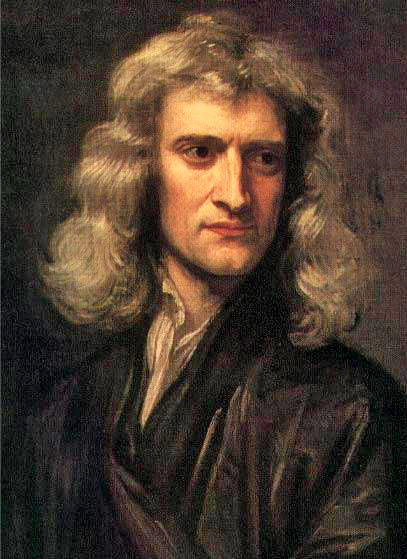
\includegraphics[scale=.25]{newton_portrait.jpg}

%\end{multicols}

}

% Section I:
\section{\sectiontitleI}

\frame{
\frametitle{\sectiontitleI}

\begin{multicols}{2}

\underline{Model:}\vspc A Swinging Pendulum \vspc

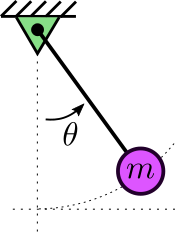
\includegraphics[scale=.6]{pendulum_fig1.png} \vspace{20mm}

\underline{Description:}\vspc A mass is suspended by a rigid link from a pin. \vspc

\underline{Assumptions:} 
\begin{itemize}
\item the mass is treated as a point mass
\item the link is rigid aand mass-less
\item the pin is frictionless
\item the air drag is negligable
\end{itemize}

\end{multicols}

}

% Section II:
\section{\sectiontitleII}

\frame{
\frametitle{\sectiontitleII}

\begin{multicols}{2}
First {\it separate} the bodies of interest to draw a {\bf free} body diagram. \ 

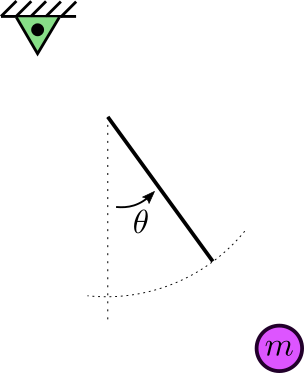
\includegraphics[scale=.5]{pendulum_fig2.png} \vspace{20mm}
\end{multicols}

Also, choose a {\R zero-pontential} reference. 
}




% Section III:
\section{\sectiontitleIII}

\frame{
\frametitle{\sectiontitleIII}

Now, identify all kinetic and potential energies present. \vspc

\underline{Kinetic Energy}\vspc
\vspace{20mm}

\underline{Potential Energy}\vspc
\vspace{30mm}

}

% Section IV:
\section{\sectiontitleIV}

\frame{
\frametitle{\sectiontitleIV}

Apply the conservation of energy. \vspc

\scalebox{1.0}{$\frac{d}{dt}\left( KE + PE \right) = \frac{d}{dt}\left(Constant\right) = 0$} 

\vspace{40mm}


}
	
% Section V:
\section{\sectiontitleV}

\frame{
\frametitle{\sectiontitleV}

Finally Re-arrange the resulting equation to get the equations of motion in a standard form.


}	
	
\end{document}





